\Chapter{Tesztelés}

Az elkészült alkalmazás Lua-ban íródott. Legelőször root jogosultságokhoz kell jussunk, akár az \texttt{su}, vagy a \texttt{sudo} parancs használatával. A program futtatása előtt meg kell győződnünk arról, hogy legalább 5.3-as Lua verzióval rendelkezünk az adott számítógépen. 

Ezt így ellenőrizhetjük:
\begin{verbatim}
# lua -v
Lua 5.4.4  Copyright (C) 1994-2022 Lua.org, PUC-Rio
\end{verbatim}

Ha esetleg nem lenne Lua feltelepítve, akkor a következő paranccsal tehetjük meg Debian/Ubuntu esetén:

\begin{verbatim}
# apt-get install lua5.4
\end{verbatim}

Ezután nincs más dolgunk, mint lefuttatni magát az alkalmazást:

\begin{verbatim}
# lua main.lua
\end{verbatim}

Ha nem rendelkezünk root jogosultságokkal, akkor az alkalmazás hibával tér vissza:

\begin{figure}[h]
\centering
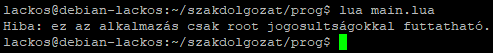
\includegraphics[scale=1]{images/root_required.png}
\caption{root jogosultságok hiányára figyelmeztető hiba}
\end{figure}

A program sikeres lefuttatása után a főmenübe érkezünk, ahol 4 lehetőségünk van:

\begin{figure}[h]
\centering
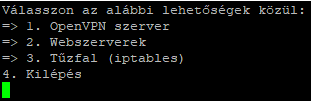
\includegraphics[scale=1]{images/main_menu.png}
\caption{a program főmenüje}
\end{figure}

A program összes menüjében úgy navigálhatunk, hogy beírjuk a sorszámot (például 1, vagy 1.) és ENTER-t nyomunk. A program törekszik arra, hogy minden instrukciót megadjon a felhasználó számára a használatára vonatkozóan. Ha hibába ütközik, kiírja a hiba kódját, továbbá lehetséges forrását.

\pagebreak

\Section{OpenVPN}

\SubSection{Konfigurálás, telepítés előtt}
Az OpenVPN menüjébe érve ezt a képet kapjuk eleinte, ha nincs feltelepítve:

\begin{figure}[h]
\centering
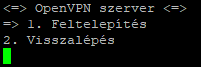
\includegraphics[scale=1]{images/openvpn_install.png}
\caption{OpenVPN főmenü - még feltelepítés előtt}
\end{figure}

Ekkor csak szimplán kiválasztjuk az egyes menüpontot, és feltelepítődik magától az OpenVPN, ekkor frissülni fog a menü erre:

\begin{figure}[h]
\centering
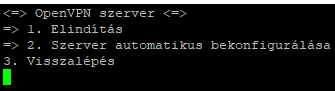
\includegraphics[scale=1]{images/openvpn_preconfig.png}
\caption{OpenVPN főmenü - még konfigurálás előtt}
\end{figure}

\SubSection{Konfigurálás, telepítés után}
Konfiguráljuk be a szervert telepítés után. Konfigurálás után a program mappájában létrejön egy openvpn mappa, amely az easyrsa programot tartalmazza. Itt található meg a saját Certificate Authority-nk, amellyel a kliensek és a szerver certificatejét, private keyét kezeli a program.

Konfigurálás után több menüpont is rendelkezésünkre fog állni:

\begin{figure}[h]
\centering
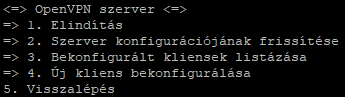
\includegraphics[scale=1]{images/openvpn_after_install.png}
\caption{OpenVPN főmenü - telepítés, konfigurálás után}
\end{figure}

A 3. menüpontban tudjuk megtekinteni a jelenleg már konfigurált klienseinket, további menüpontok nyílnak onnan: vissza tudjuk vonni egy kliens hozzáférését az OpenVPN szerverhez, továbbá ki tudjuk iratni a kliens konfigját. A kliens konfigja teljesen kimásolható, csak az IP-címet kell átírni benne a saját szerverünk IP-címére. Mindent tartalmaz beágyazva (a certificatet, kulcsfájlokat, tls-crypt fájlt, satöbbit).
Ha egy kliens hozzáférését visszavonjuk, akkor a hozzá generált certificatek, kulcsok revokeolásra kerülnek, és a kliens neve újra felhasználható lesz.


A 4. menüpontban tudunk új klienst létrehozni, két adatot kér be: a kliens nevét, amellyel azonosíthatjuk és egy jelszót a privát kulcsához. A jelszó megadása biztonsági okokból kötelező. A kliens nevének egyedinek kell lennie, duplikáció nem megengedett.

\pagebreak

\Section{Webszerverek}
A webszerverek menüjébe érve választhatunk \texttt{Apache} és \texttt{nginx} között is. A két webszerver kezelőfelülete között nincs különbség, teljesen egy kódstruktúrára is épülnek, ezért egyben fogom bemutatni őket. Értelemszerűen ha nincs feltelepítve az adott webszerver, akkor a telepítést fogja felajánlani:

\begin{figure}[h]
\centering
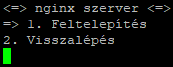
\includegraphics[scale=1]{images/web_before_install.png}
\caption{Webszerver főmenü - telepítés előtt}
\end{figure}

Telepítés után a következő menüpontokat láthatjuk:

\begin{figure}[h]
\centering
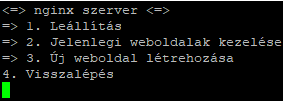
\includegraphics[scale=1]{images/web_after_install.png}
\caption{Webszerver főmenü - telepítés után}
\end{figure}

A 2. menüpontban tudjuk kezelni a meglévő weboldalainkat, amint kiválasztottunk egyet, utána további menüpontokhoz jutunk:

\begin{itemize}
	\item a legelső menüpont a weboldal törlését jelenti, ez kitörli a weboldal konfigurációját és magát a weboldalt tartalmazó www mappát is
	\item a második menüpont pedig az SSL certificatek certbot általi generálását szolgálja. 
	Több lehetőség is van a certificatek generálására: HTTP-01 challenge, amely egy fájl automatikus elhelyezésével működik; vagy DNS-01 challenge, amelynél a saját névszerverünknél (DNS szerverünknél) beállítások módosítására is szükségünk van. A DNS-01-et akkor célszerű választani, ha valamiért a 80-as portot nem tudjuk használni.
\end{itemize}

A 3. menüpontban tudunk új weboldalakat létrehozni, ehhez magára csak a weboldal címére van szükség. Automatikusan létrehozza a program a weboldal konfigurációját, a weboldal www-dirjét, továbbá egy index.html fájlt:

\begin{figure}[h]
\centering
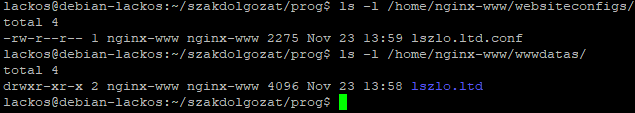
\includegraphics[scale=1]{images/website_config_dir_examples.png}
\caption{Weboldal konfigurációjának helye, weboldal www-dirje nginx esetén}
\end{figure}

\pagebreak

\Section{iptables}

\SubSection{Feltelepítés előtt}
Az iptables menüpontot választva, ha nincs még feltelepítve a frontend, akkor felajánlja a program:

\begin{figure}[h]
\centering
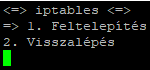
\includegraphics[scale=1]{images/iptables_before_install.png}
\caption{iptables feltelepítése előtt}
\end{figure}

\SubSection{Feltelepítés után}

Feltelepítés után több menüpont is a szemünk elé tárul:

\begin{figure}[h]
\centering
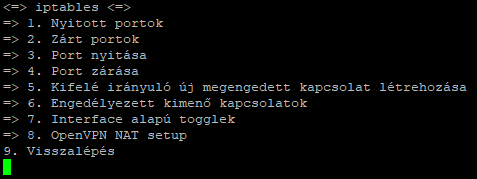
\includegraphics[scale=1]{images/iptables_mainmenu.png}
\caption{iptables főmenüje}
\end{figure}

A menüpontok magukért beszélnek. Minden menüpont kiválasztása után felugrik egy interface kiválasztó felület, amellyel az adott funkcionalitást leszűkíthetjük egy interfacera.

\begin{figure}[h]
\centering
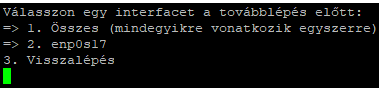
\includegraphics[scale=1]{images/iptables_interface_select.png}
\caption{iptables - interface választása}
\end{figure}

Ha az összes interfacet választjuk, akkor a program szigorúan azt kezeli, amikor egy szabály ténylegesen mindenre érvényes. Ez azt jelenti iptables esetén, hogy nem adunk meg interfacet hozzá (nem manuálisan adja hozzá a program minden egyes interfacehoz az adott szabályt). Ez azt jelenti, hogy az adott szabály az interfacek változása esetén is megmarad. 

Érdemes ezt figyelembevenni a program használatakor, mert például a nyitott portok lehet, hogy az "all" (vagyis az összes) interfacera vonatkozóan vannak kinyitva, és így nem mutatja ki másik interface-n való nyitott portok lekérdezésekor.

\pagebreak

\texttt{Port nyitáskor} három adatra lesz szükségünk az interface kiválasztása után: a \texttt{protokollra} (tcp/udp/all), a \texttt{port számára} és a \texttt{bejövő IP-címre}. Ha a bejövő IP-cím üresen marad, bármely IP tud csatlakozni erre a portra.

\texttt{Port záráskor} is három adatra lesz szükségünk az interface kiválasztása után: a \texttt{protokollra} (tcp/udp/all), a \texttt{port számára} és a \texttt{bejövő IP-címre}. Ha a bejövő IP-cím üresen marad, mindegyik IP le lesz tiltva erről a portról.

\texttt{Kifelé irányuló új kapcsolat engedélyezésekor} is három adat lesz szükséges: \\a \texttt{protokoll} (tcp/udp/all), a \texttt{port számára} és a \texttt{külső IP-címre}. Ha a port száma üresen marad, akkor a teljes IP-címet engedélyezi kifelé irányuló új kapcsolatként.

A "\texttt{nyitott portok}", "\texttt{zárt portok}" és "\texttt{engedélyezett kimenő kapcsolatok}", továbbá a "\texttt{OpenVPN NAT setup}" menüpont alatt tudjuk ellenőrzni a már meglévő beállításainkat. Ezekben a menüpontokban tudjuk törölni is a már létrehozott szabályokat is.

Az interface alapú togglek menüpontban van két, a működés szempontjából nagyon fontos beállítás: itt lehet beállítani, hogy minden bejövő, vagy kimenő kapcsolat szűrve legyen-e. Ha egy adott portot kinyitunk, és nem tiltjuk le az összes nem engedélyezett bejövő kapcsolatot, akkor a port nyitás szabály jelenleg épp nem lesz effektív (azonban ígyis megmarad a későbbiekre). Szintén ez vonatkozik a kimenő kapcsolatokra is: ha hozzáadunk egy engedélyezett kimenő kapcsolatot, de nem tiltjuk le a nem engedélyezett kimenő kapcsolatokat, akkor a szabály nem lesz effektív.

Az \texttt{OpenVPN NAT setup} menüpontban tudunk NAT-szabályokat létrehozni az\\ OpenVPN szerverünkhöz, ha feltelepítettük és bekonfiguráltuk a program segítségével. Automatikusan felismeri, ha már van meglétező NAT szabályunk létrehozva, kilistázza azokat és törölni is tudjuk őket. 

\SubSection{Minden forgalom átirányítása OpenVPN szerveren keresztül}

A NAT bekonfigurálása után, ha minden forgalmat át akarunk irányítani az\\ OpenVPN szerverünkön keresztül a kliens felől, ne felejtsük el a \texttt{\detokenize{net.ipv4.ip_forward}} flaget beállítani a Linux szerveren. Alapértelmezésként a program csak kommentként adja hozzá azt az option-t az OpenVPN szerver konfigurációjához, amely átirányít minden forgalmat a VPN csatornára, ezt kell uncommentelnünk:

\begin{verbatim}
# nano /etc/openvpn/server_openvpn_serv.conf # ez az alapértelmezett
## elérése az OpenVPN szerver konfigurációnak
\end{verbatim}

Maga a beállítás:
\begin{verbatim}
#push "redirect-gateway def1 bypass-dhcp"
\end{verbatim}

A \detokenize{net.ipv4.ip_forward} flaget pedig a sysctl.conf szerkesztésével tudjuk bekapcsolni:
\begin{verbatim}
# nano /etc/sysctl.conf
# sysctl -p
\end{verbatim}
Ha nincs a flag a fájlban, írjuk bele: "\detokenize{net.ipv4.ip_forward = 1}" ha van, akkor pedig kapcsoljuk be (írjuk át 1-re).


